%%%%%%%%%%%%%%%%%%%%%%%%%%%%%%%%%%%%%%%%%%%%%%%%%%%%%%%%%%%%%%%%%%%%%%%%%%%%%%%%
\exercice{Décomposition en signaux usuels}
%%%%%%%%%%%%%%%%%%%%%%%%%%%%%%%%%%%%%%%%%%%%%%%%%%%%%%%%%%%%%%%%%%%%%%%%%%%%%%%%

Soit la fonction porte $p_a(t)$ définie graphiquement de la façon suivante :

\tikzsetnextfilename{exercice_2-chap0-ext}
\begin{center}
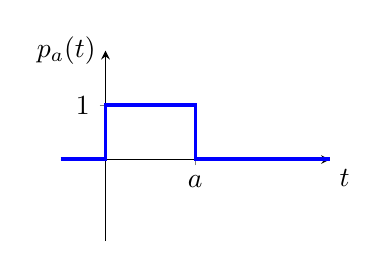
\begin{tikzpicture}[baseline=0]
   \begin{axis}[
        height=4cm,
        width=5cm,
        axis x line=center,
        axis y line=center,
        xmin=-1,
        xmax=5,
        ymin=-1.5,
        ymax=2.0,
        xlabel={$t$},
        ylabel={$p_a(t)$},
        xlabel style={below right},
        ylabel style={left},
        yticklabels={1},
        ytick={1},
        y tick label style={anchor=east},
        xticklabels={$a$},
        xtick={2},
        x tick label style={anchor=north},
        ]
        \addplot [very thick,color=blue,const plot] coordinates 
        {(-1,0.01) (0,0.01) (0,1) (2,1)  (2,0.01) (5,0.01) };
        \end{axis}
\end{tikzpicture}
\end{center}

\question{}
\textbf{Déterminer $p_a(t)$ (la fonction porte) à l'aide de fonctions échelons. 
et donner sa transformée de Laplace.}
\newline

Soit la fonction $u_a(t)$ définie graphiquement de la façon suivante :

\tikzsetnextfilename{exercice_3-chap0-ext}
\begin{center}
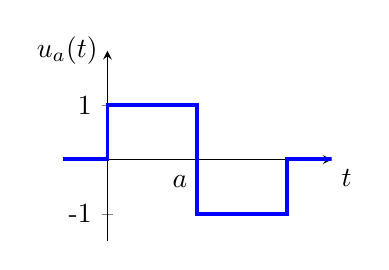
\begin{tikzpicture}[baseline=0]
   \begin{axis}[
   height=4cm,
   width=5cm,
      axis x line=center,
        axis y line=center,
        xmin=-1,
        xmax=5,
        ymin=-1.5,
        ymax=2.0,
        xlabel={$t$},
        ylabel={$u_a(t)$},
        xlabel style={below right},
        ylabel style={left},
        yticklabels={-1,1},
        ytick={-1,1},
        y tick label style={anchor=east},
        xticklabels={$a$},
        xtick={2},
        x tick label style={below left},
        ]
        \addplot [very thick,color=blue,const plot] coordinates 
        {(-1,0.01) (0,0.01) (0,1) (2,1)  (2,-1) (4,-1) (4,0.01) (5,0.01)  };
        \end{axis}
\end{tikzpicture}
\end{center}

\question{}
\textbf{Déterminer $u_a(t)$ en fonction de $p_a(t)$ et donner sa 
transformée de Laplace.}
\newline

Soit la fonction $g_0(t)$ définie graphiquement de la façon suivante :

\tikzsetnextfilename{exercice_4-chap0-ext}
\begin{center}
\begin{tikzpicture}[baseline=0]
   \begin{axis}[
   height=4cm,
   width=5cm,
      axis x line=center,
        axis y line=center,
        xmin=-1,
        xmax=5,
        ymin=-1.5,
        ymax=2.0,
        xlabel={$t$},
        ylabel={$g_0(t)$},
        xlabel style={below right},
        ylabel style={left},
        yticklabels={$E$},
        ytick={1},
        y tick label style={left},
        xticklabels={$\dfrac{T}{2}$,$T$},
        xtick={2,4},
        x tick label style={below},
        ]
        \addplot [very thick,color=blue,domain=-1:0, samples=101]{0.05};
        \addplot [very thick,color=blue,domain=0:2, samples=101]{0.5*x};
        \addplot [very thick,color=blue,domain=2:4, samples=101]{-0.5*x+2};
        \addplot [very thick,color=blue,domain=4:5, samples=101]{0.05};
        \end{axis}
\end{tikzpicture}
\end{center}

\question{}
\textbf{Déterminer $g_0(t)$ en fonction de $u_a(t)$ et donner sa 
transformée de Laplace.}

\newpage
%%%%%%%%%%%%%%%%%%%%%%%%%%%%%%%%%%%%%%%%%%%%%%%%%%%%%%%%%%%%%%%%%%%%%%%%%%%%%%%%
\exercice{Décomposition en signaux usuels (2)}
%%%%%%%%%%%%%%%%%%%%%%%%%%%%%%%%%%%%%%%%%%%%%%%%%%%%%%%%%%%%%%%%%%%%%%%%%%%%%%%%

\question{}
\textbf{Déterminer la transformée de Laplace des signaux suivants en 
décomposant le signal en somme d'échelons et de rampes; $g(t)$ étant un signal
périodique.}

\tikzsetnextfilename{exercice_4-1-chap0-ext}
\begin{center}
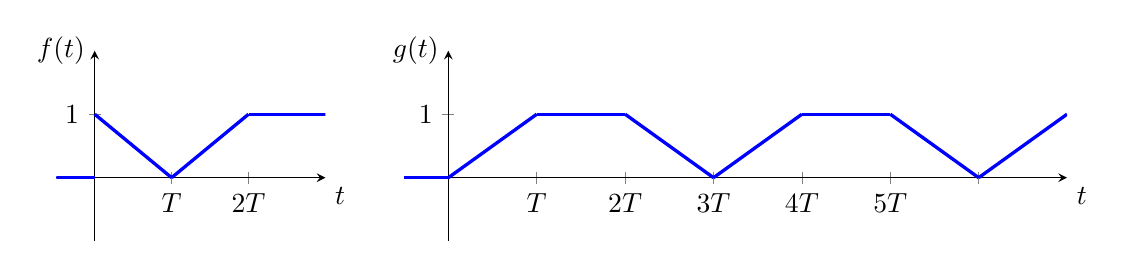
\begin{tikzpicture}[baseline=0]
   \begin{axis}[
        name=first,   
        height=4cm,
        width=5cm,
        axis x line=center,
        axis y line=center,
        xmin=-1,
        xmax=6,
        ymin=-1,
        ymax=2.0,
        xlabel={$t$},
        ylabel={$f(t)$},
        xlabel style={below right},
        ylabel style={left},
        yticklabels={1},
        ytick={1},
        y tick label style={left},
        xticklabels={0,$T$,$2T$},
        xtick={0,2,4},
        x tick label style={below},
        ]
        \addplot [very thick,color=blue,domain=-1:0, samples=101]{0};
        \addplot [very thick,color=blue,domain=0:2, samples=101]{-0.5*x+1};
        \addplot [very thick,color=blue,domain=2:4, samples=101]{0.5*x-1};
        \addplot [very thick,color=blue,domain=4:6, samples=101]{1};
        \end{axis}
   \begin{axis}[
        at=(first.east),anchor=west,xshift=1cm,
        height=4cm,
        width=10cm,
        axis x line=center,
        axis y line=center,
        xmin=-1,
        xmax=14,
        ymin=-1,
        ymax=2.0,
        xlabel={$t$},
        ylabel={$g(t)$},
        xlabel style={below right},
        ylabel style={left},
        yticklabels={1},
        ytick={1},
        y tick label style={left},
        xticklabels={0,$T$,$2T$,$3T$,$4T$,$5T$},
        xtick={0,2,4,6,8,10,12},
        x tick label style={below},
       ]
        \addplot [very thick,color=blue,domain=-1:0, samples=101]{0};
        \addplot [very thick,color=blue,domain=0:2, samples=101]{0.5*x};
        \addplot [very thick,color=blue,domain=2:4, samples=101]{1};
        \addplot [very thick,color=blue,domain=4:6, samples=101]{-0.5*x+3};
        \addplot [very thick,color=blue,domain=6:8, samples=101]{0.5*x-3};
        \addplot [very thick,color=blue,domain=8:10, samples=101]{1};
        \addplot [very thick,color=blue,domain=10:12, samples=101]{-0.5*x+6};
        \addplot [very thick,color=blue,domain=12:14, samples=101]{0.5*x-6};
   \end{axis}
\end{tikzpicture}
\end{center}

%%%%%%%%%%%%%%%%%%%%%%%%%%%%%%%%%%%%%%%%%%%%%%%%%%%%%%%%%%%%%%%%%%%%%%%%%%%%%%%%
\exercice{\'Etude d'équations différentielles}
%%%%%%%%%%%%%%%%%%%%%%%%%%%%%%%%%%%%%%%%%%%%%%%%%%%%%%%%%%%%%%%%%%%%%%%%%%%%%%%%

Un système linéaire est décrit par les équations différentielles suivantes :
$$
\devi{s(t)}{2} + 110 \devi{s(t)}{} + 1000 s(t) = \devi{x(t)}{} + 30 x(t)
$$
et 
$$
\devi{x(t)}{} + x(t) = K e(t) 
$$

$e(t)$ est l'entrée du système, la sortie $s(t)$ et $x(t)$ est une variable
interne. On se place dans les conditions d'Heaviside (c.a.d conditions 
initiales nulles).\newline

\question{}
\textbf{\'Ecrire ces équations dans le domaine de Laplace (avec 
$p\in\mathbb{C}$ la variable complexe).}

\question{}
\textbf{Tracer le schéma fonctionnel complet du système.}

\question{}
\textbf{Déterminer la fonction de transfert du système.}
\newline

On sollicite le système avec un échelon $e(t)=E_0 u(t)$

\question{}
\textbf{Déterminer la valeur finale de la sortie et la tangente à l'origine.}

\question{}
\textbf{Déterminer la sortie $s(t)$ et tracer le signal.}

\exercice{Fonction de transfert, réponse temporelle}

\question{}
\textbf{Pour chacunes des équations différentielles suivantes, 
déterminer la fonction de transfert $H(p) = S(p)/E(p)$, les valeurs initiales
et finales ainsi que leurs réponses temporelles $s(t)$.}

\begin{itemize}
\item[\textbf{(1)}] $\devi{s(t)}{} + 2s(t) = e(t) $ avec $s(0)=2$ 
                    et $e(t) = e^{-t}$
\item[\textbf{(2)}] $\devi{s(t)}{2} + 3 \devi{s(t)}{} + 2s(t) 
                    = \devi{e(t)}{} + e(t)$ 
                    avec $\devi{s(0)}{}=s(0)=0$ et $e(t) = e^{-3t}$
\item[\textbf{(3)}] $\devi{s(t)}{2} + 2\devi{s(t)}{} + s(t)  = e(t)$ 
                    avec $\devi{s(0)}{}=s(0)=0$ et $e(t) = e^{-2t}$
\item[\textbf{(4)}] $\devi{s(t)}{2} + \devi{s(t)}{} + s(t) = e(t)$ 
                    avec $\devi{s(0)}{}=s(0)=0$ et $e(t) = 1$
\end{itemize}

%%%%%%%%%%%%%%%%%%%%%%%%%%%%%%%%%%%%%%%%%%%%%%%%%%%%%%%%%%%%%%%%%%%%%%%%%%%%%%%%
\exercice{Transformée de Laplace d'une fonction périodique}
%%%%%%%%%%%%%%%%%%%%%%%%%%%%%%%%%%%%%%%%%%%%%%%%%%%%%%%%%%%%%%%%%%%%%%%%%%%%%%%%

Nous rappelons que dans le cas générale, 
la transformée de Laplace d'une fonction causale et périodique $f(t)$ de 
période $T$ est donné par :
$$
F(p) = \dfrac{F_0(p)}{1-e^{-Tp}}
$$
où $F_0(p)$ est la transformée de Laplace du motif $f_0(t)$ égal à $f(t)$ 
sur le segment $[0,T]$ et nulle partout ailleurs.

\question{}
\textbf{Déterminer la transformée de Laplace $F(p)$ de la fonction 
        temporelle $f(t)$ causale et périodique, définie par la figure 
        ci-dessous :}

\begin{center}
    \tikzsetnextfilename{exercice_1-chap0-ext}
    \begin{tikzpicture}
        \begin{axis}[
        height=5cm,
        width=0.75\textwidth,  
        axis x line=center,
        axis y line=center,
        xmin=-1,
        xmax=16,
        ymin=-1.5,
        ymax=1.5,
        xlabel={$t$},
        ylabel={$f(t)$},
        xlabel style={below right},
        ylabel style={above left},
        yticklabels={$-E$,$E$},
        ytick={-1,1},
        y tick label style={anchor=east},
        xticklabels={$\dfrac{T}{2}$,$T$,$2T$},
        xtick={2,4,8},
        x tick label style={below},
        extra x ticks={6},
        extra x tick labels={$\dfrac{3T}{2}$},
        extra x tick style={
        xticklabel style={above},}
        ]
        \addplot [very thick,color=blue,domain=0:2  ,samples=101]
        {0.5*x};
        \addplot [very thick,color=blue,domain=2:6  ,samples=101]
        {-0.5*x+2};
        \addplot [very thick,color=blue,domain=6:10 ,samples=101]
        {0.5*x-4};
        \addplot [very thick,color=blue,domain=10:14,samples=101]
        {-0.5*x+6};
        \end{axis}
    \end{tikzpicture}
\end{center}

Pour répondre à la question on pourra s'aider des résultats de 
l'exercice~\ref{exe-1_chap0} pour progressivement construire le motif de 
base de cette fonction périodique à savoir $f_0(t)=f(t)$ pour 
$0\leq t\leq2T$ en fonction de $g_0(t)$.

%%%%%%%%%%%%%%%%%%%%%%%%%%%%%%%%%%%%%%%%%%%%%%%%%%%%%%%%%%%%%%%%%%%%%%%%%%%%%%%%
\exercice{Cartes des pôles et zéros}
%%%%%%%%%%%%%%%%%%%%%%%%%%%%%%%%%%%%%%%%%%%%%%%%%%%%%%%%%%%%%%%%%%%%%%%%%%%%%%%%

\question{}
Tracer la carte des pôles et zéros des fonctions de transferts suivantes:
\begin{itemize}
    \item[(a)] $H_1(p)=\dfrac{4p}{p^3+2p^2+8p+16}$
    \item[(b)] $H_2(p)=\dfrac{(p+1)}{(p^2+2p+2)(p+4)}$
    \item[(c)] $H_3(p)=\dfrac{(p+1)}{(p^2+2p+1)(p^2+p+0.5)}$
\end{itemize}
%%%%%%%%%%%%%%%%%%%%%%%%%%%%%%%%%%%%%%%%%%%%%%%%%%%%%%%%%%%%%%%%%%%%%%%%%%%%%%%%
%%%%%%%%%%%%%%%%%%%%%%%%%%%%%%%%%%%%%%%%%%%%%%%%%%%%%%%%%%%%%%%%%%%%%%%%%%%%%%%%
%%%%%%%%%%%%%%%%%%%%%%%%%%%%%%%%%%%%%%%%%%%%%%%%%%%%%%%%%%%%%%%%%%%%%%%%%%%%%%%%
%%%%%%%%%%%%%%%%%%%%%%%%%%%%%%%%%%%%%%%%%%%%%%%%%%%%%%%%%%%%%%%%%%%%%%%%%%%%%%%%
%exercice_chap0.tex
